% Created 2015-01-04 dom 10:46
\documentclass[xcolor={usenames,svgnames,dvipsnames}]{beamer}
\usepackage[utf8]{inputenc}
\usepackage[T1]{fontenc}
\usepackage{fixltx2e}
\usepackage{graphicx}
\usepackage{longtable}
\usepackage{float}
\usepackage{wrapfig}
\usepackage{rotating}
\usepackage[normalem]{ulem}
\usepackage{amsmath}
\usepackage{textcomp}
\usepackage{marvosym}
\usepackage{wasysym}
\usepackage{amssymb}
\usepackage{hyperref}
\tolerance=1000
\usepackage{color}
\usepackage{listings}
\usepackage{gensymb}
\usepackage{amsmath}
\AtBeginSection[]{\begin{frame}[plain]\tableofcontents[currentsection,hideallsubsections]\end{frame}}
\AtBeginSubsection[]{\begin{frame}[plain]\tableofcontents[currentsubsection,sectionstyle=show/shaded,subsectionstyle=show/shaded/hide]\end{frame}}
\lstset{keywordstyle=\color{blue}, commentstyle=\color{gray!90}, basicstyle=\ttfamily\small, columns=fullflexible, breaklines=true,linewidth=\textwidth, backgroundcolor=\color{gray!23}, basewidth={0.5em,0.4em}, literate={á}{{\'a}}1 {ñ}{{\~n}}1 {é}{{\'e}}1 {ó}{{\'o}}1 {º}{{\textordmasculine}}1}
\usepackage[emulate=units]{siunitx}
\sisetup{per=fraction, fraction=nice, decimalsymbol=comma}
\newunit{\wattpeak}{Wp}
\newunit{\watthour}{Wh}
\newunit{\amperehour}{Ah}
\usepackage{mathpazo}
\usefonttheme{serif}
\usecolortheme{rose}
\usetheme{Goettingen}
\hypersetup{colorlinks=true, linkcolor=Blue, urlcolor=Blue, breaklinks=true}
\bibliographystyle{plain}
\setbeamercolor{alerted text}{fg=red!50!black} \setbeamerfont{alerted text}{series=\bfseries}
\usetheme{default}
\author{Oscar Perpiñán Lamigueiro (UPM)}
\date{}
\title{Radiación Solar}
\hypersetup{
  pdfkeywords={},
  pdfsubject={},
  pdfcreator={Emacs 24.3.1 (Org mode 8.2.7c)}}
\begin{document}

\maketitle


\section{Naturaleza de la radiación solar}
\label{sec-1}

\begin{frame}[label=sec-1-0-1]{Irradiancia e Irradiación}
\begin{description}
\item[{Irradiancia}] es la densidad de \emph{potencia} de radiacion solar
incidente en una superficie.

\begin{itemize}
\item Unidades: $\si{\watt\per\meter\squared},\,\si{\kilo\watt\per\meter\squared}$
\end{itemize}

\item[{Irradiación}] es la densidad de \emph{energía} de radiación solar
incidente en una superficie.

\begin{itemize}
\item Unidades: $\si{\watthour\per\meter\squared},\,\si{\kilo\watthour\per\meter\squared}$
\end{itemize}
\end{description}
\end{frame}

\begin{frame}[label=sec-1-0-2]{Radiación Extra-atmosférica}
\begin{itemize}
\item La radiación que alcanza la superficie de la atmósfera es radiación
directa del Sol.

\item \alert{Constante solar} $B_{0}=\SI{1367}{\watt\per\meter\squared}$
   (irradiancia solar sobre la superficie normal al vector solar en límite superior de la atmósfera terrestre)

\item \alert{Irradiancia extra-atmosférica}

\begin{itemize}
\item $B_{0}(0)=B_{0}\cdot\epsilon_{0}\cdot\cos\theta_{zs}$

\item $B_{0d}(0)=-\frac{T}{\pi}B_{0}\epsilon_{0}\cdot\left(\omega_{s}\sin\phi\sin\delta+\cos\delta\cos\phi\sin\omega_{s}\right)$
      ($\omega_{s}$ en radianes)
\end{itemize}
\end{itemize}
\end{frame}

\begin{frame}[label=sec-1-0-3]{Radiación Extra-atmosférica}
\begin{itemize}
\item Es posible demostrar que el \alert{promedio mensual} de esta irradiación
diaria \alert{coincide numericamente} con el valor de irradiación diaria
correspondiente a los denominados \alert{días promedios}, días en los que
la declinación correspondiente coincide con el promedio mensual

\item Por tanto, podemos calcular el valor medio mensual de la irradiación
diaria extra-atmosférica con el valor de la declinación de uno de los
doce días promedio.
\end{itemize}

\begin{center}
\begin{tabular}{lrrrrrr}
Mes & Ene & Feb & Mar & Abr & May & Jun\\
\hline
$d_n$ & 17 & 45 & 74 & 105 & 135 & 161\\
\hline
Mes & Jul & Ago & Sep & Oct & Nov & Dic\\
\hline
$d_n$ & 199 & 230 & 261 & 292 & 322 & 347\\
\end{tabular}
\end{center}
\end{frame}

\begin{frame}[label=sec-1-0-4]{Interacción de la radiación con la atmósfera}
\begin{itemize}
\item \alert{Disminución} de la radiación incidente en la superficie terrestre
(reflexión en nubes)

\item \alert{Modificación de las características espectrales} de la radiación
(absorción por vapor de agua, ozono y CO2)

\item \alert{Modificación de la distribución espacial} (dispersión por
partículas)

\begin{itemize}
\item Difusión de Rayleigh (longitud de onda mucho mayor que tamaño de
partícula) - Capas altas - Color Azul

\item Difusión de Mie (longitud de onda de magnitud similar a tamaño de
partícula) - Capas bajas

\item Difusión no selectiva (longitud de onda mucho menor que tamaño de
partícula)
\end{itemize}
\end{itemize}
\end{frame}

\begin{frame}[label=sec-1-0-5]{Componentes de la radiación solar}
\begin{itemize}
\item \alert{Radiación Directa}. (B)

\begin{itemize}
\item Linea recta con el Sol.
\end{itemize}

\item \alert{Radiación Difusa}. (D)

\begin{itemize}
\item Procedente de todo el cielo salvo el Sol

\item Rayos dispersados por la atmósfera.

\item Anisotrópica, proceso estocástico.
\end{itemize}

\item \alert{Radiación del albedo}. (R, AL)

\begin{itemize}
\item Procedente del suelo (reflejada)
\end{itemize}

\item \alert{Radiación Global:} $G=B+D+R$
\end{itemize}
\end{frame}

\begin{frame}[label=sec-1-0-6]{Cómo se escribe}
\begin{block}{Forma, tiempo, lugar}
\begin{description}
\item[{Forma+Tiempo+Lugar:}] Irradiancia directa (forma) horaria (tiempo)
en el plano del generador (lugar)

\item[{Promedios:}] Media mensual (periodo) de la irradiación global
(forma) diaria (tiempo)

\item[{Lugar:}] (Orientación, Inclinación)

(0=Horizontal)

(n=Normal)

(I=Plano del generador)
\end{description}
\end{block}
\end{frame}

\begin{frame}[label=sec-1-0-7]{Cómo se escribe}
\begin{block}{Forma, tiempo, lugar}
\[Forma_{tiempo,promedio}(lugar)\]

\[G_{d,m}(0)\]

\[D_{h}(\alpha,\beta)\]

\[B_{0d}(n)\]

\[B(\beta)\]
\end{block}
\end{frame}

\begin{frame}[label=sec-1-0-8]{Caracterización de la atmósfera}
\begin{itemize}
\item \alert{Masa de aire}:

\begin{itemize}
\item Relación entre camino recorrido por rayos directos del Sol a
través de la atmósfera hasta la superficie receptora y el que
recorrerían en caso de incidencia vertical (AM=1)

\item $AM=1/\cos\theta_{zs}$
\end{itemize}

\item \alert{Índice de claridad}

\begin{itemize}
\item Relación entre la radiación global en el plano horizontal y la
radiación extra-atmosférica en el plano horizontal

\item El índice de claridad \alert{no depende de las variaciones debidas al
movimiento aparente del sol}.

\item $K_{Tm}=\frac{G_{d,m}(0)}{B_{0d,m}(0)}$ (mensual)
\end{itemize}
\end{itemize}
\end{frame}

\begin{frame}[label=sec-1-0-9]{Índice de claridad}
\begin{description}
\item[{$K_{T}$:}] índice de claridad instantáneo. $K_{T}=G/B_{0}$

\item[{$K_{Td}$:}] índice de claridad diario. $K_{Td}=G_{d}/B_{0d}$

\item[{$K_{Tm}$:}] índice de claridad mensual. $K_{Tm}=G_{m}/B_{0m}=G_{d,m}/B_{0d,m}$

\item[{$K_{Ta}$:}] índice de claridad anual. $K_{Ta} = G_{a}/B_{0a} = \dots$
\end{description}
\end{frame}

\section{Cálculo de componentes de radiación solar}
\label{sec-2}

\begin{frame}[label=sec-2-0-1]{Radiación como proceso estocástico}
\begin{itemize}
\item La \alert{distribución de valores} que presenta la radiación solar durante un periodo está \alert{determinada por el valor promedio de la radiación durante ese periodo}.

\begin{itemize}
\item Por ejemplo, conocer la media mensual de la radiación solar diaria en un determinado lugar permite saber cómo se comportará la radiación diaria durante ese mes
\end{itemize}

\item El índice de claridad para un día concreto \alert{sólo está influido} por el índice de claridad del \alert{día anterior}.
\end{itemize}
\end{frame}

\begin{frame}[label=sec-2-0-2]{Estimación de Directa y Difusa}
\begin{itemize}
\item Establecer una \alert{relación entre la fracción difusa} de la radiación horizontal ($F_{D}=\frac{D(0)}{G(0)}$) y \alert{el índice de claridad}.

\item \alert{Correlación negativa} (a mayor índice de claridad, menor componente difusa)

\item \alert{Correlación independiente de la latitud} (validez cuasi-universal)
\end{itemize}
\end{frame}

\begin{frame}[label=sec-2-0-3]{Correlaciones $F_{D}$ y $K_{T}$: Ecuación de Page}
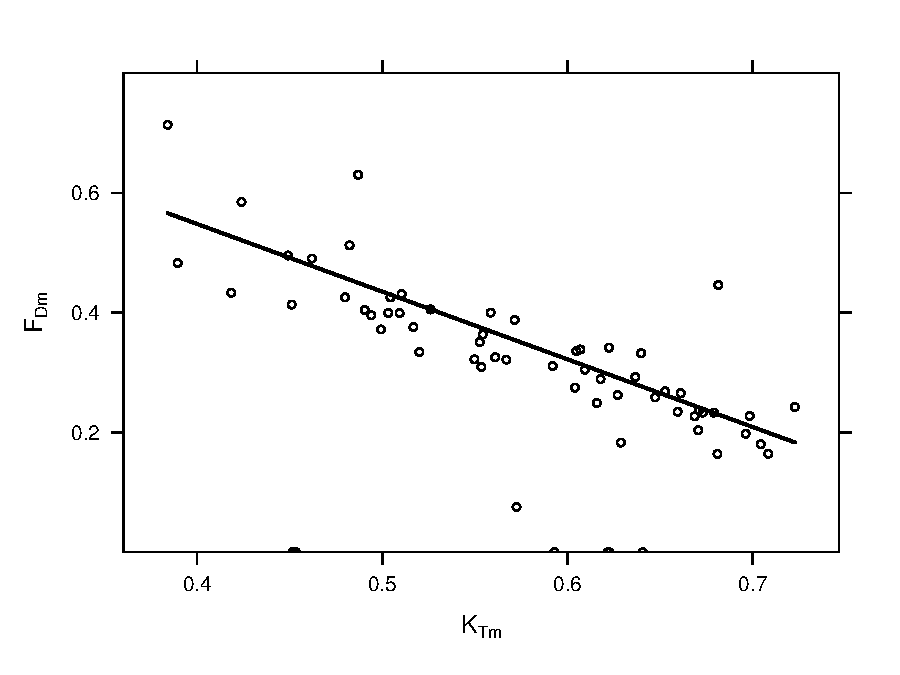
\includegraphics[width=.9\linewidth]{../figs/FdKtMensual.pdf}

\[F_{Dm}=1-1.13\cdot K_{Tm}\]
\end{frame}

\begin{frame}[label=sec-2-0-4]{Correlaciones $F_{D}$ y $K_{T}$}
Ejemplo: en un lugar con $G_{d,m}(0) = \SI{3150}{\watthour\per\meter\squared}$ en un mes con $B_{o,dm}(0) = \SI{4320}{\watthour\per\meter\squared}$  será:

\begin{itemize}
\item $K_{Tm}=\frac{3150}{4320}=0.73$

\item Según la correlación de Page, $F_{Dm}=1-1.13\cdot0.73=0.175$

\item $D_{d,m}(0)=0.175\cdot3150=\SI{551.6}{\watthour\per\meter\squared}$

\item $B_{d,m}(0)=3150-551.6=\SI{2598,4}{\watthour\per\meter\squared}$
\end{itemize}
\end{frame}

\begin{frame}[label=sec-2-0-5]{Correlaciones $F_{D}$ y $K_{T}$: Collares-Pereira y Rabl}
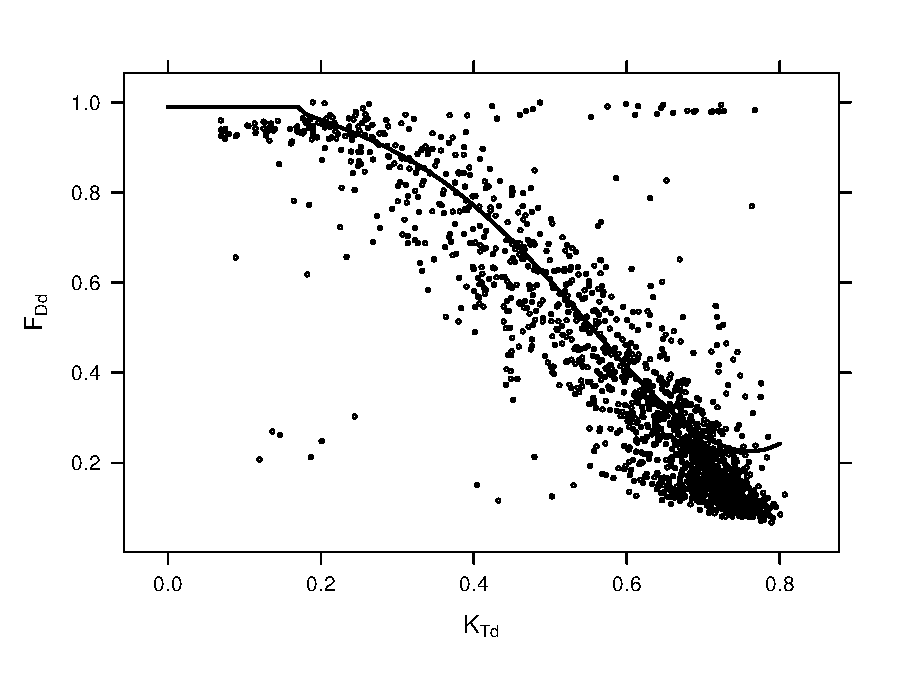
\includegraphics[width=.9\linewidth]{../figs/FdKtDiario.pdf}
{\scriptsize \[
F_{Dd} = \begin{cases}
  0.99 & K_{Td} \leq 0.17\\
  1.188 - 2.272 \cdot K_{Td} + 9.473 \cdot K_{Td}^{2} - 21.856 \cdot K_{Td}^{3} + 14.648 \cdot K_{Td}^{4} & K_{Td} > 0.17
\end{cases}
\]
}
{\scriptsize \par}
\end{frame}

\begin{frame}[label=sec-2-0-6]{Estimación de Directa y Difusa}
\begin{description}
\item[{Calcular}] las componentes directa y difusa de la radiación solar del:

\begin{itemize}
\item Mes de Septiembre (día 261) en un lugar con latitud $\phi=\ang{40}\mathrm{N}$ y con media mensual de irradiación global diaria horizontal
$G_{d,m}(0)=\SI{2700}{\watthour\per\meter\squared}$.
\end{itemize}
\end{description}
\end{frame}


\section{Cálculo de radiación sobre generadores}
\label{sec-3}


\begin{frame}[label=sec-3-0-1]{Irradiancia sobre superficies arbitrarias}
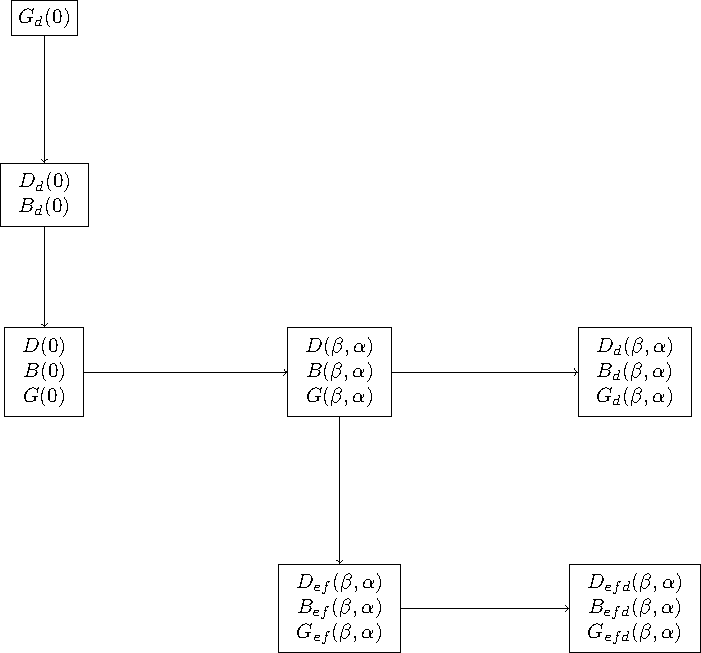
\includegraphics[width=.9\linewidth]{../figs/ProcedimientoCalculoRadiacionInclinada.pdf}
\end{frame}

\subsection{Irradiancia a partir de irradiación diaria}
\label{sec-3-1}

\begin{frame}[label=sec-3-1-1]{Estimación de Irradiancia a partir de Irradiación diaria}
\begin{itemize}
\item La irradiación durante una hora coincide con el valor medio de la irradiancia durante esa hora.

\item La variación solar durante una hora es baja: valor de irradiancia equivalente a valor de irradiación.

\item Relación entre irradiancia e irradiación extra-terrestre deducible teóricamente:
\end{itemize}

\[\frac{B_{o}(0)}{B_{0d}(0)}=\frac{\pi}{T}\cdot\frac{\cos(\omega)-\cos(\omega_{s})}{\omega_{s}\cdot\cos(\omega_{s})-\sin(\omega_{s})}\]
\end{frame}

\begin{frame}[label=sec-3-1-2]{Estimación de Irradiancia a partir de Irradiación diaria}
\[r_{D}=\frac{D(0)}{D_{d}(0)}=\frac{B_{o}(0)}{B_{0d}(0)}\]

\[r_{G}=\frac{G(0)}{G_{d}(0)}=r_{D}\cdot\left(a+b\cdot\cos(\omega)\right)\]

\[a=0.409-0.5016\cdot\sin(\omega_{s}+\frac{\pi}{3})\]

\[b=0.6609+0.4767\cdot\sin(\omega_{s}+\frac{\pi}{3})\]
\end{frame}


\begin{frame}[label=sec-3-1-3]{Estimación de Irradiancia a partir de Irradiación diaria}
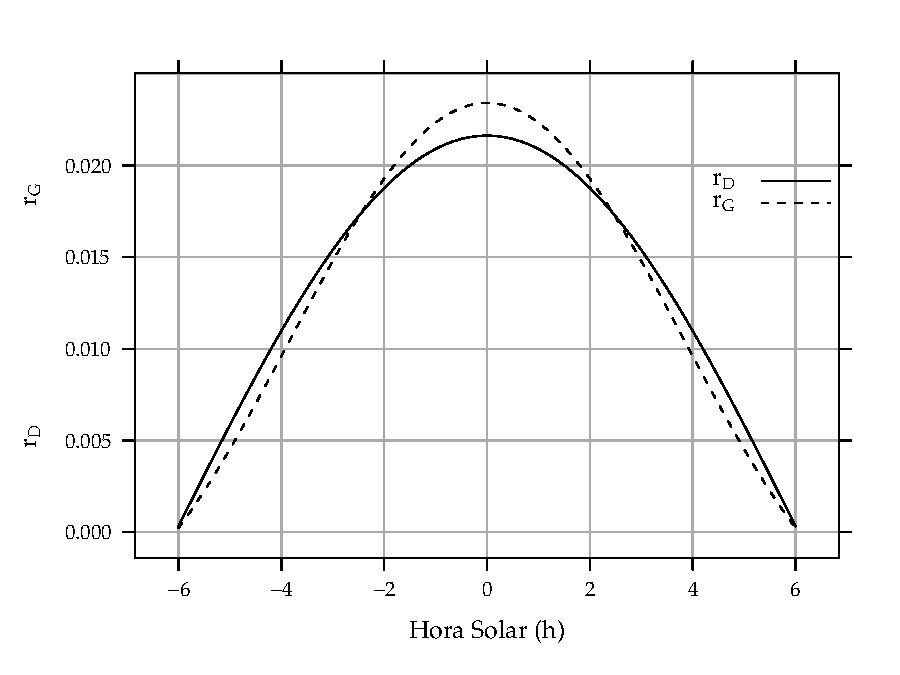
\includegraphics[width=.9\linewidth]{../figs/RgRd.pdf}
\end{frame}

\begin{frame}[label=sec-3-1-4]{Estimación de Irradiancia a partir de Irradiación diaria}
\begin{description}
\item[{Calcular}] la irradiancia global y la irradiancia difusa en el plano horizontal

\begin{itemize}
\item 2 horas antes del mediodía del día 261 en un lugar con latitud $\phi=\ang{40}\mathrm{N}$ y con media mensual de irradiación global diaria horizontal $G_{d,m}(0)=\SI{2700}{\watthour\per\meter\squared}$.
\end{itemize}
\end{description}
\end{frame}

\subsection{Transformación al plano del generador}
\label{sec-3-2}

\begin{frame}[label=sec-3-2-1]{Irradiancia Directa}
\[B(\beta,\alpha)=B(0)\cdot\frac{\max(0,\cos(\theta_{s}))}{\cos(\theta_{zs})}\]
\end{frame}

\begin{frame}[label=sec-3-2-2]{Factor de visión para Difusa}
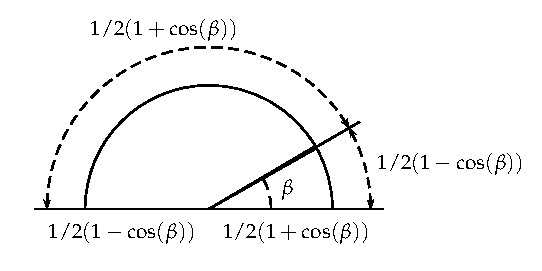
\includegraphics[width=.9\linewidth]{../figs/AnguloVisionCielo.pdf}

\[D(\beta,\alpha)=\intop_{\Omega}L(\theta_{z},\psi)\cdot\cos(\theta_{z}^{'})d\Omega\]
\end{frame}

\begin{frame}[label=sec-3-2-3]{Irradiancia Difusa isotrópica}
\[L(\theta_{z},\psi)=cte.\]

\[D(\beta,\alpha)=D(0)\cdot\frac{1+\cos(\beta)}{2}\]
\end{frame}

\begin{frame}[label=sec-3-2-4]{Irradiancia Difusa Anisotrópica}
\[D(\beta,\alpha) = D^{I}(\beta,\alpha)+D^{C}(\beta,\alpha)\]
\[D^{I}(\beta,\alpha) = D(0) \cdot (1-k_{1}) \cdot \frac{1 + \cos(\beta)}{2}\]
\[D^{C}(\beta,\alpha) = D(0) \cdot k_{1} \cdot \frac{\max(0,\cos(\theta_{s}))}{\cos(\theta_{zs})}\]
\[k_{1} & = & \frac{B(0)}{B_{0}(0)}\]
\end{frame}

\begin{frame}[label=sec-3-2-5]{Irradiancia de Albedo}
\[R(\beta,\alpha)=\rho\cdot G(0)\cdot\frac{1-\cos(\beta)}{2}\]

\[\rho=0.2\]
\end{frame}

\begin{frame}[label=sec-3-2-6]{Irradiancia sobre plano inclinado}
\begin{description}
\item[{Calcular}] la irradiancia difusa, directa, de albedo y global, en

\begin{itemize}
\item Un generador inclinado $\ang{30}$ y orientado al Sur, 2 horas antes del mediodía del día 261 en un lugar con latitud  $\phi=\ang{40}\mathrm{N}$ y con media mensual de irradiación global diaria horizontal $G_{d,m}(0)=\SI{2700}{\watthour\per\meter\squared}$.
\end{itemize}
\end{description}
\end{frame}


\subsection{Pérdidas angulares y por suciedad}
\label{sec-3-3}

\begin{frame}[label=sec-3-3-1]{Radiación directa}
\[B_{ef}(\beta,\alpha)=B(\beta,\alpha)\cdot\left[\frac{T_{sucio}(0)}{T_{limpio}(0)}\right]\cdot (1-FT_{B}(\theta_{s}))\]

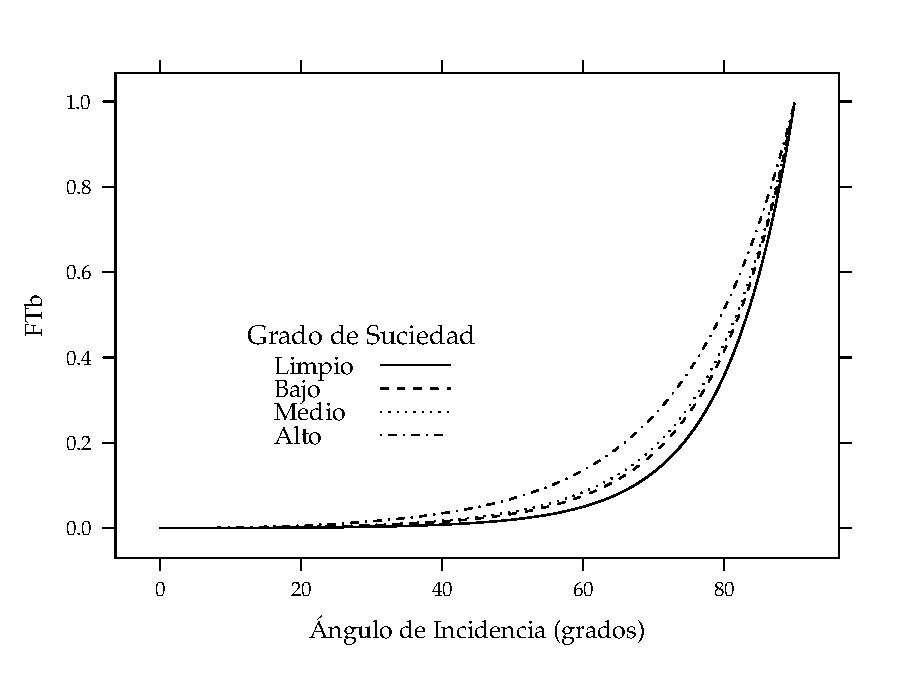
\includegraphics[width=.9\linewidth]{../figs/Suciedad.pdf}
\end{frame}

\begin{frame}[label=sec-3-3-2]{Difusa y Albedo}
\begin{aligned}

D_{ef}^{iso}(\beta,\alpha) & = & D^{iso}(\beta,\alpha)\cdot\left[\frac{T_{sucio}(0)}{T_{limpio}(0)}\right]\cdot(1-FT_{D}(\beta))\\

D_{ef}^{cir}(\beta,\alpha) & = & D^{cir}(\beta,\alpha)\cdot\left[\frac{T_{sucio}(0)}{T_{limpio}(0)}\right]\cdot(1-FT_{B}(\theta_{s}))\\

R_{ef}(\beta,\alpha) & = & R(\beta,\alpha)\cdot\left[\frac{T_{sucio}(0)}{T_{limpio}(0)}\right]\cdot(1-FT_{R}(\beta))

\end{aligned}
\end{frame}

\begin{frame}[label=sec-3-3-3]{Coeficientes}
\begin{center}
\begin{tabular}{lrrr}
Grado de Suciedad & $\frac{T_{sucio}(0)}{T_{limpio}(0)}$ & $a_{r}$ & $c_{2}$\\
\hline
Limpio & 1 & 0.17 & -0.069\\
Bajo & 0.98 & 0.20 & -0.054\\
Medio & 0.97 & 0.21 & -0.049\\
Alto & 0.92 & 0.27 & -0.023\\
\end{tabular}
\end{center}
\end{frame}

\begin{frame}[label=sec-3-3-4]{Pérdidas anuales}
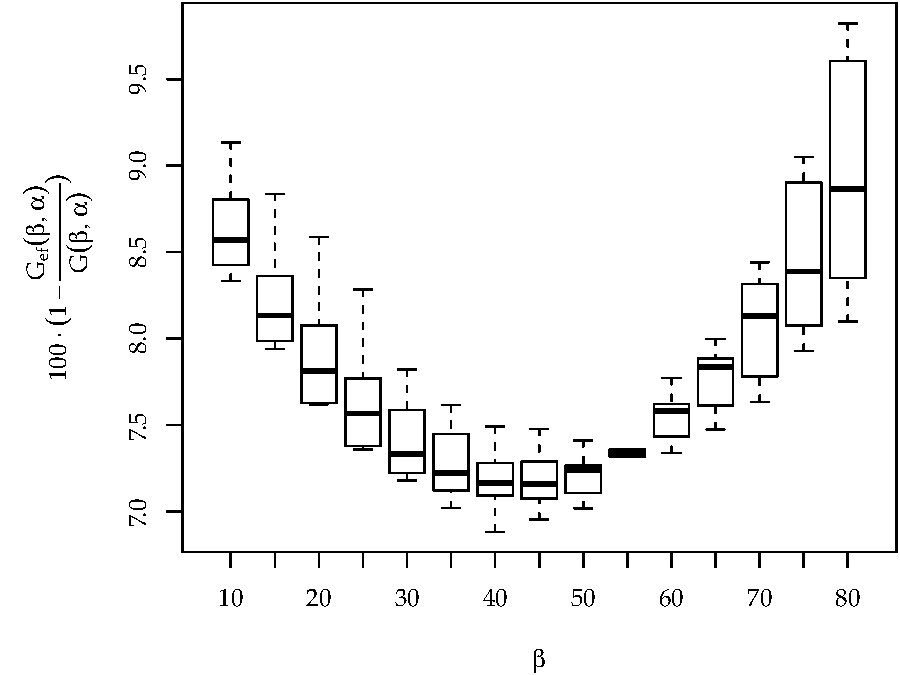
\includegraphics[width=.9\linewidth]{../figs/GefVSG.pdf}
\end{frame}

\section{Radiación Efectiva según tipologías}
\label{sec-4}



\begin{frame}[label=sec-4-0-1]{Radiación en Sistema estático}
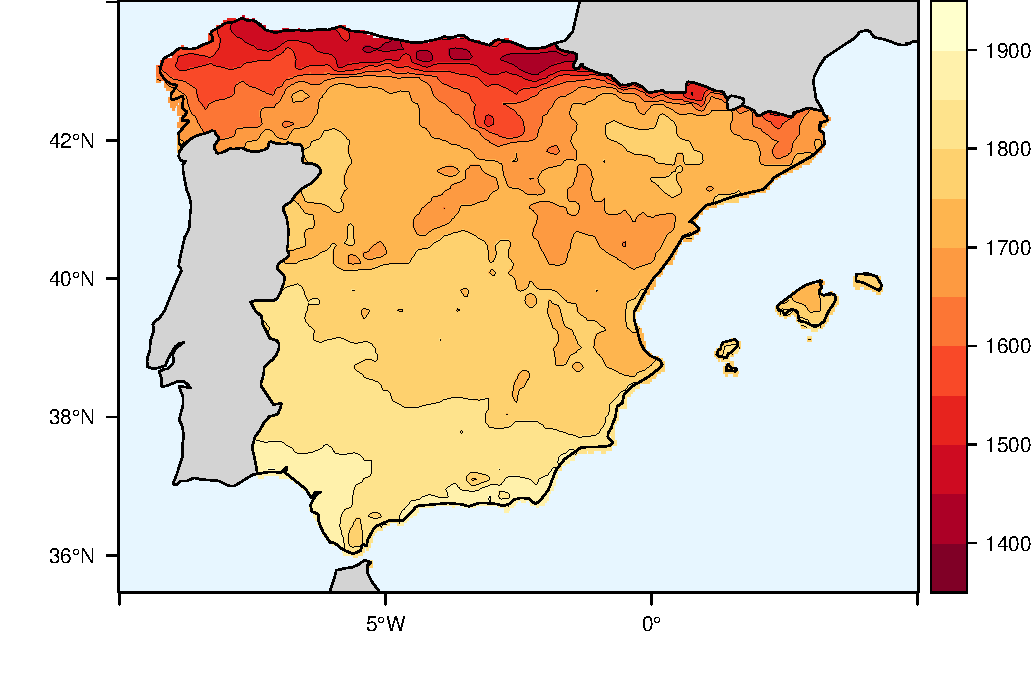
\includegraphics[width=.9\linewidth]{../figs/FixedKrig.pdf}
\end{frame}



\begin{frame}[label=sec-4-0-2]{Radiación en Seguimiento Eje Horizontal}
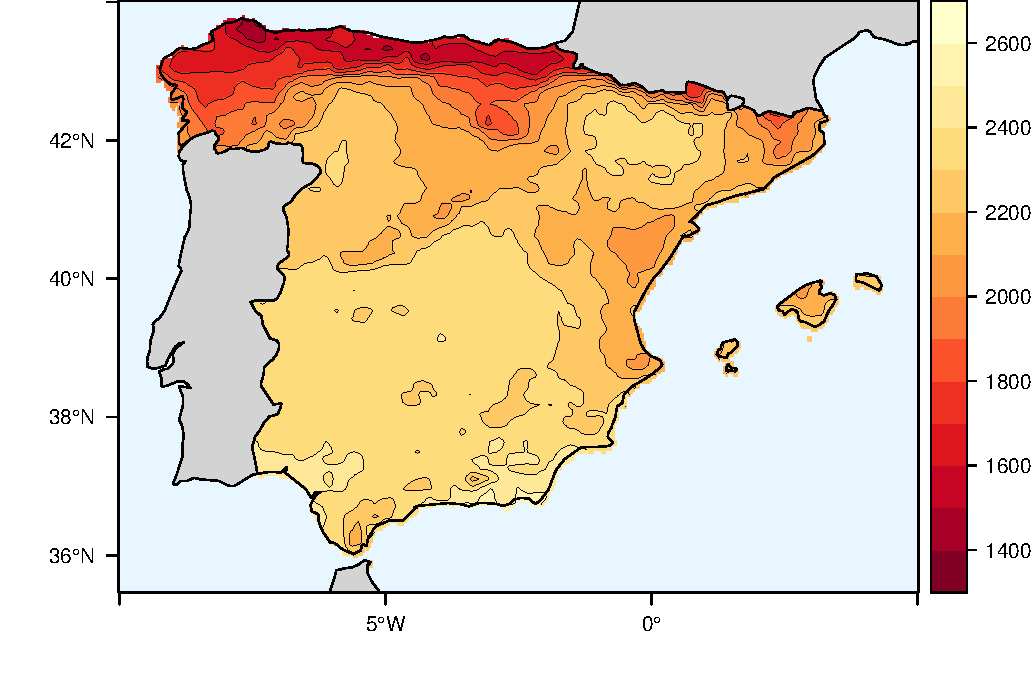
\includegraphics[width=.9\linewidth]{../figs/HorizKrig.pdf}
\end{frame}



\begin{frame}[label=sec-4-0-3]{Radiación en Seguimiento Doble Eje}
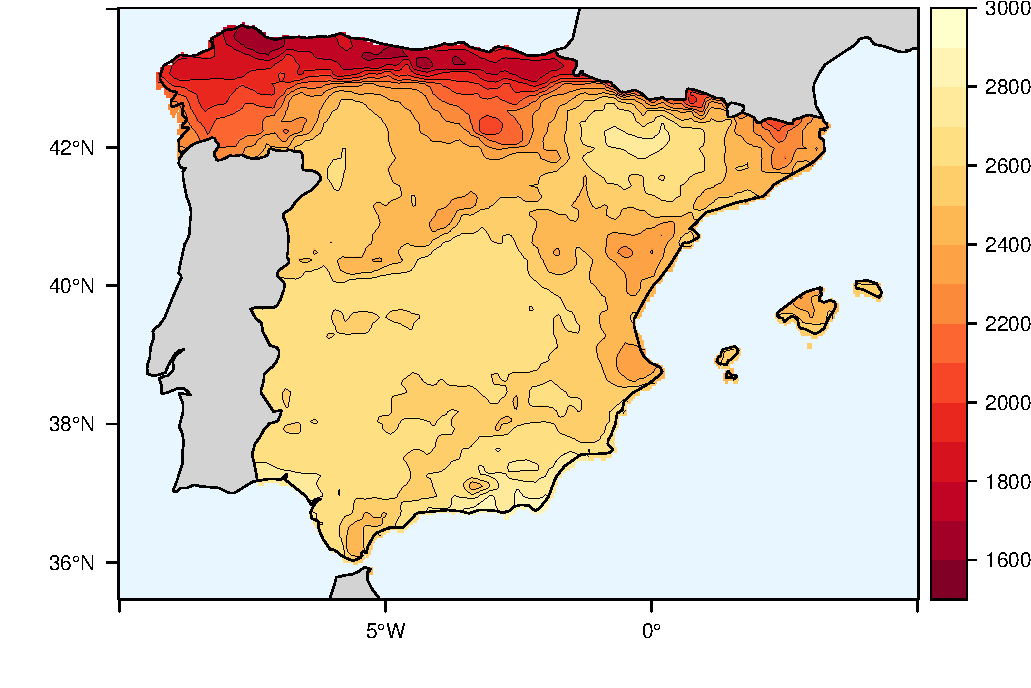
\includegraphics[width=.9\linewidth]{../figs/TwoKrig.pdf}
\end{frame}

\subsection{Comparación entre tipologías}
\label{sec-4-1}



\begin{frame}[label=sec-4-1-1]{Comparación Doble Eje-Estática}
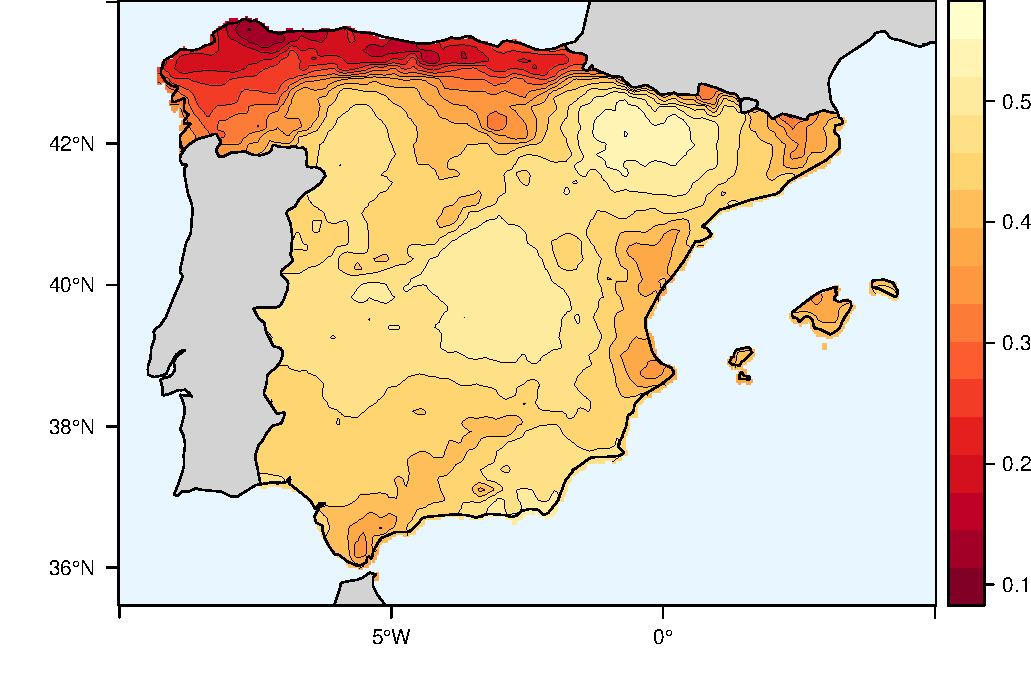
\includegraphics[width=.9\linewidth]{../figs/TwoFixed.pdf}
\end{frame}



\begin{frame}[label=sec-4-1-2]{Comparación Doble Eje - Horizontal}
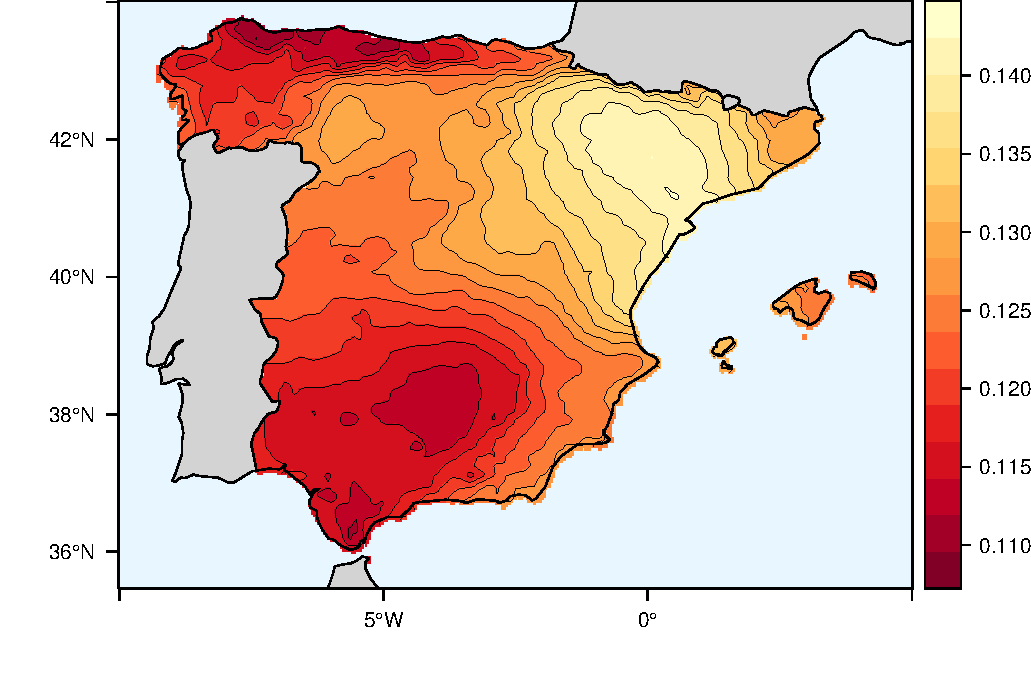
\includegraphics[width=.9\linewidth]{../figs/TwoHoriz.pdf}
\end{frame}



\begin{frame}[label=sec-4-1-3]{Comparación Eje Horizontal - Estática}
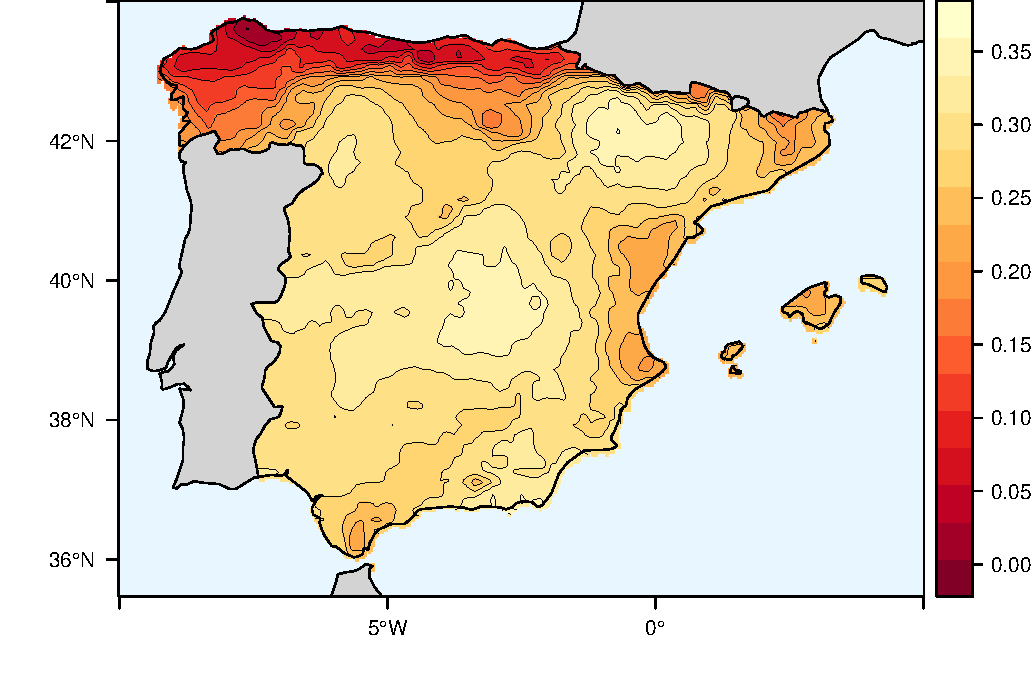
\includegraphics[width=.9\linewidth]{../figs/HorizFixed.pdf}
\end{frame}



\begin{frame}[label=sec-4-1-4]{Comparación Eje Horizontal - Estática}
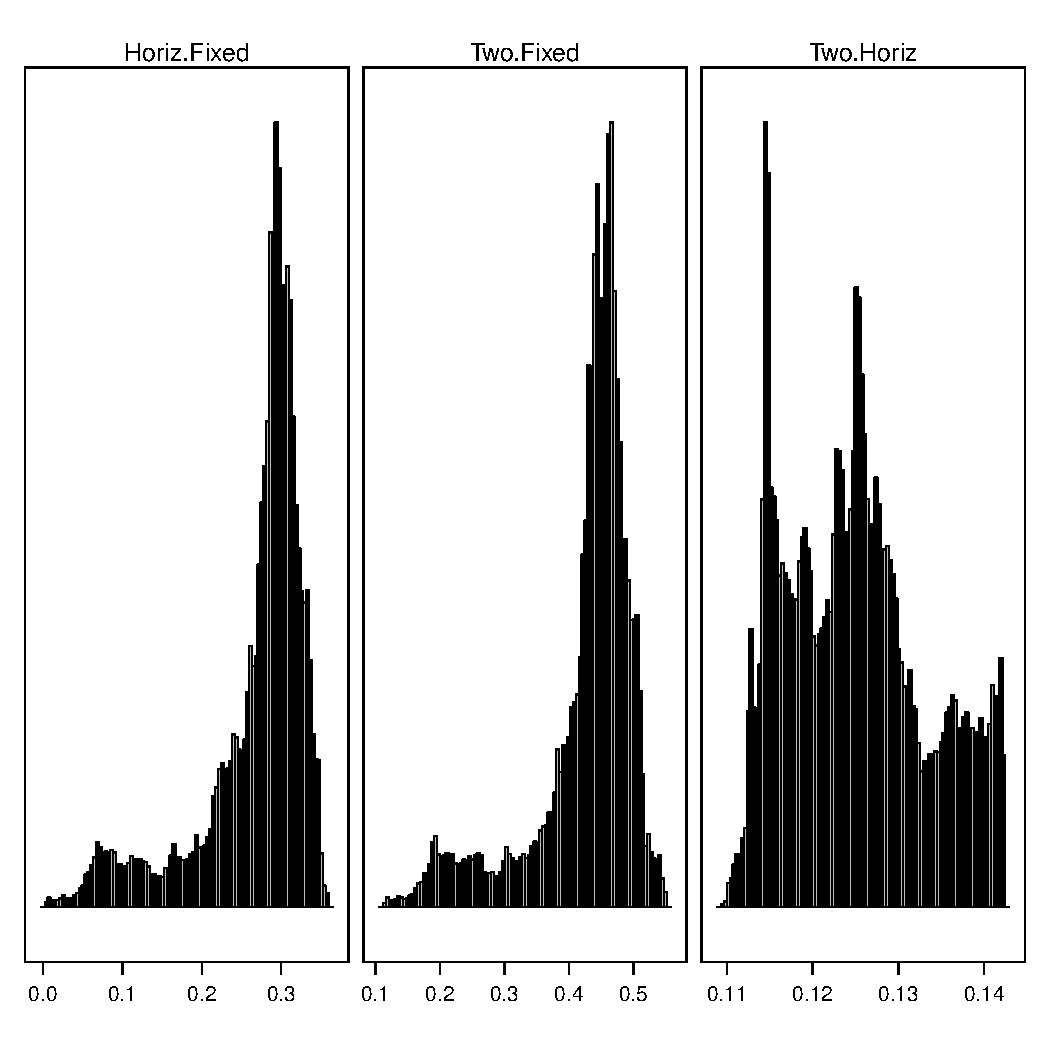
\includegraphics[width=.9\linewidth]{../figs/compSystems.pdf}

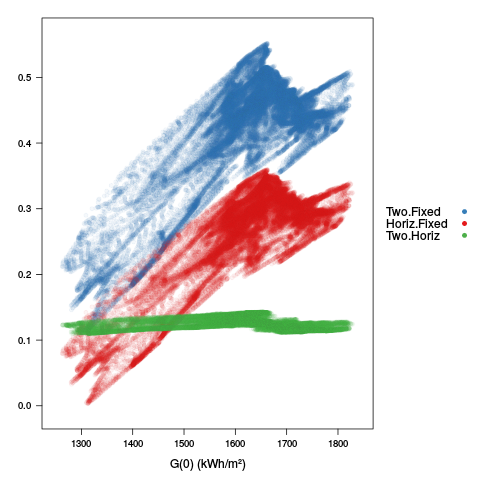
\includegraphics[width=.9\linewidth]{../figs/compSystemsG0.pdf}
\end{frame}

\section{Aplicación a Sistemas estáticos}
\label{sec-5}

\subsection{Ángulo de inclinación óptimo}
\label{sec-5-1}

\begin{frame}[label=sec-5-1-1]{Inclinación Optima Estática}
\[\left|\phi\right|-\beta\approx10\degree\]

\[\beta_{opt}=3.7+0.69\cdot|\phi|\]
\end{frame}

\begin{frame}[label=sec-5-1-2]{Sensibilidad al desapuntamiento}
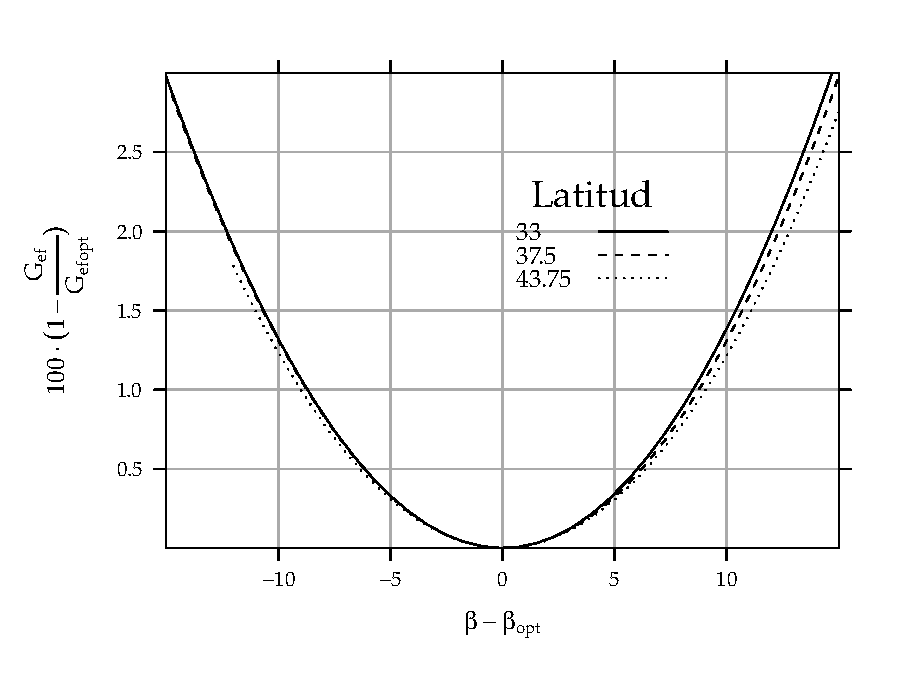
\includegraphics[width=.9\linewidth]{../figs/PerdidasInclinacionOptima.pdf}
\end{frame}

\begin{frame}[label=sec-5-1-3]{Radiación para inclinación óptima}
\[\frac{G_{d,a}(0)}{G_{d,a}(\beta_{opt})}=1-4.46\cdot10^{-4}\cdot\beta_{opt}-1.19\cdot10^{-4}\cdot\beta_{opt}^{2}\]
\end{frame}

\begin{frame}[label=sec-5-1-4]{Cálculo de Radiación Efectiva}
\[
\frac{G_{efd,a}(\beta,\alpha)}{G_{d,a}(\beta_{opt})} = g_{1}\cdot(\beta-\beta_{opt})^{2}+g_{2}\cdot(\beta-\beta_{opt})+g_{3}
\]

\[
g_{i} = g_{i1}|\alpha|^{2}+g_{i2}|\alpha|+g_{i3}
\]

\begin{center}
\begin{tabular}{lrrr}
 & $i=1$ & $i=2$ & $i=3$\\
\hline
$g_{1i}$ & $8\cdot10^{-9}$ & $3.8\cdot10^{-7}$ & $-1.218\cdot10^{-4}$\\
$g_{2i}$ & $-4.27\cdot10^{-7}$ & $8.2\cdot10^{-6}$ & $2.892\cdot10^{-4}$\\
$g_{3i}$ & $-2.5\cdot10^{-5}$ & $-1.034\cdot10^{-4}$ & $0.9314$\\
\end{tabular}
\end{center}
\end{frame}

\begin{frame}[label=sec-5-1-5]{Cálculo para estática}
\begin{description}
\item[{Calcular}] la irradiación anual efectiva que incide en

\begin{itemize}
\item Un generador orientado al Sur e inclinado $\ang{20}$ en un lugar con latitud $\ang{30}\mathrm{N}$ y una media anual de la irradiación global diaria en el plano horizontal de $\SI{5250}{\watthour\per\meter\squared}$, suponiendo una suciedad media.
\end{itemize}

\item[{Calcular}] la irradiación anual efectiva que incide en

\begin{itemize}
\item Un generador desorientado $\ang{20}$ del Sur e inclinado $\ang{40}$ en un lugar con latitud $\ang{50}\mathrm{N}$ y una media anual de la irradiación global diaria en el plano horizontal de $\SI{5250}{\watthour\per\meter\squared}$, suponiendo una suciedad media.
\end{itemize}
\end{description}
\end{frame}
% Emacs 24.3.1 (Org mode 8.2.7c)
\end{document}